\documentclass{article}

\title{Internet Video Streaming}
\date{2023-02-28}
\author{Manuel Cadeddu}
\usepackage[italian]{babel}
\usepackage{amsmath}
\usepackage{graphicx}
\usepackage{subcaption}
\usepackage{setspace}
\usepackage{xcolor} 


\begin{document}
	\pagenumbering{arabic}
	\maketitle
	\newpage
	\doublespacing
	\tableofcontents
	\singlespacing
	\newpage

	\section{Segnali Audio e Voce}

		\subsection{Introduzione}
			Un'\textbf{onda acustica} (suono) è una variazione della pressione dell'aria nel tempo. La sua \textbf{ampiezza} indentifica il "volume" del suono ed è misurata come differenza tra la pressione locale e quella dell'onda sonora. La sua \textbf{frequenza} identifica il fonema, ovvero il suono ("a", "b"). Solo una parte delle onde sonore sono udibili dall'uomo (es. non percepiamo infra/ultra-suoni) e solo una parte di queste è riproducibile tramite le corde vocali (umane).
			\\Come possiamo notare dal seguente grafico, gli umani riescono a sentire suoni con frequenze fino a \textbf{20 KHz} e fino a \textbf{130 dB}. I suoni riproducibili sono di frequenze comprese tra i \textbf{100} e i \textbf{5-7 KHz} e tra i \textbf{25} e i \textbf{70 dB}. Notare che per musica si intende quella prodotta ad esempio da strumenti.
			\begin{figure}[ht!]
				\centering{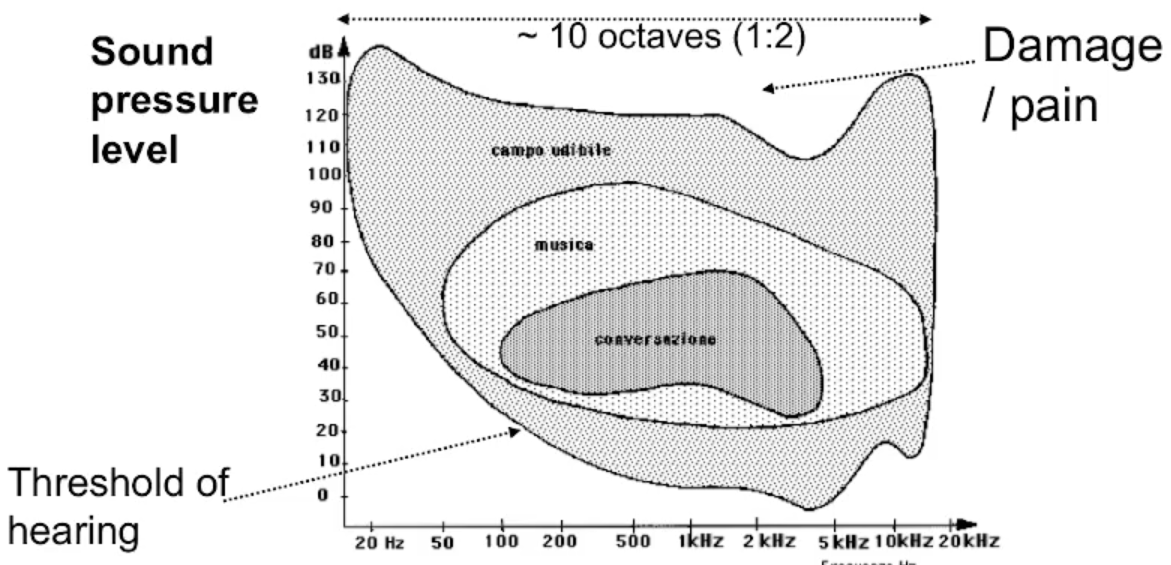
\includegraphics[width=12cm,height=5cm,keepaspectratio]{01_1.png}}
			\end{figure}
			\\I suoni che superano la soglia superiore del Sound Pressure Level (volume del suono, dato dalla variazione di pressione) causano dolore/danni all'orecchio umano, quelli inferiori alla soglia di udibilità invece non sono udibili.
			\\Dal precedente grafico possiamo fare diverse osservazioni:
			\begin{itemize}
				\item le due scale sono logaritmiche (ogni punto equivale ad un "x val" rispetto al precedente): sono udibili suoni con frequenza maggiore fino a 20k volte rispetto alla frequenza minima e suoni con un valore fino a $10^{13}$ volte maggiore del minimo udibile;
				\item \textit{SPL} = $10\log_{10}(P/P_{0})$
				\begin{itemize}
					\item $P_{0}$ è il valore minimo percettibile a 1 KHz
				\end{itemize}
				\item il suono udibile è di circa 10 ottave (raddoppiamento di frequenza);
				\item quando si lavora in dB si hanno sempre misure relative (non assolute);
				\item la miglior frequenza per scoltare suoni bassi è a circa 3 KHz.
			\end{itemize}
	
		\newpage
		\subsection{Converione A/D}
			La conversione analogico/digitale consiste nella trasformazione di un segnale continuo in uno discreto. La conversione avviene attraverso diverse fasi:
			\begin{enumerate}
				\item cattura del segnale analogico (es. con microfono);
				\item \textbf{campionamento};
				\item \textbf{quantizzazione}.
			\end{enumerate}

			\subsubsection{Campionamento}
				Il campionamento consiste nella cattura del segnale in precisi istanti di tempo (solitamente ad intervalli regolari). In questo modo si passsa da segnale a tempo continuo a segnale a tempo discreto.
				\begin{figure}[ht!]
					\centering{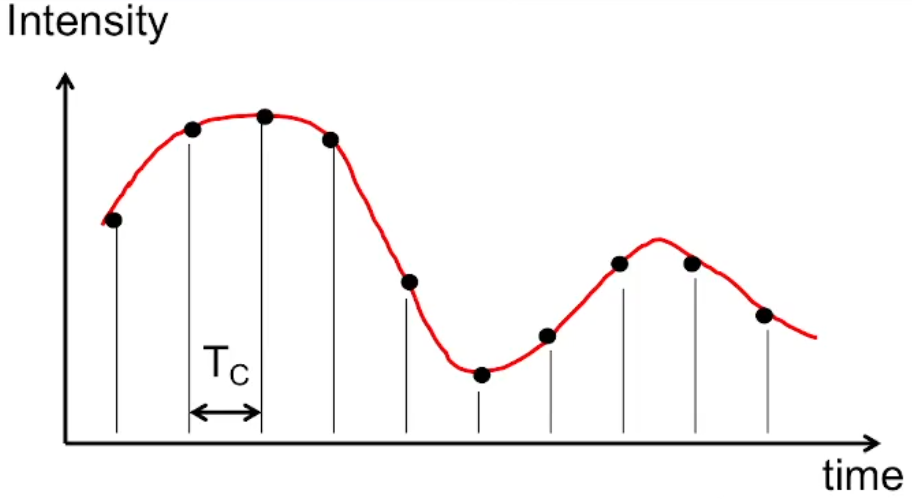
\includegraphics[width=12cm,height=3.5cm,keepaspectratio]{01_2.png}}
				\end{figure}
				\\Nota:
				\begin{itemize}
					\item per poter ricostruire il segnale analogico da quello campionato è necessario che la frequenza di campionamento \textit{$f_{c} = 1/T_{c}$} sia almeno \textit{$2 * f_{max}$} del segnale che deve essere campionato (\textbf{Teorema di Nyquist}).
				\end{itemize}

			\subsubsection{Quantizzazione}	
				La quantizzazione consiste nella mappatura dei valori continui del segnale analogico in valori discreti.
				\begin{figure}[ht!]
					\centering{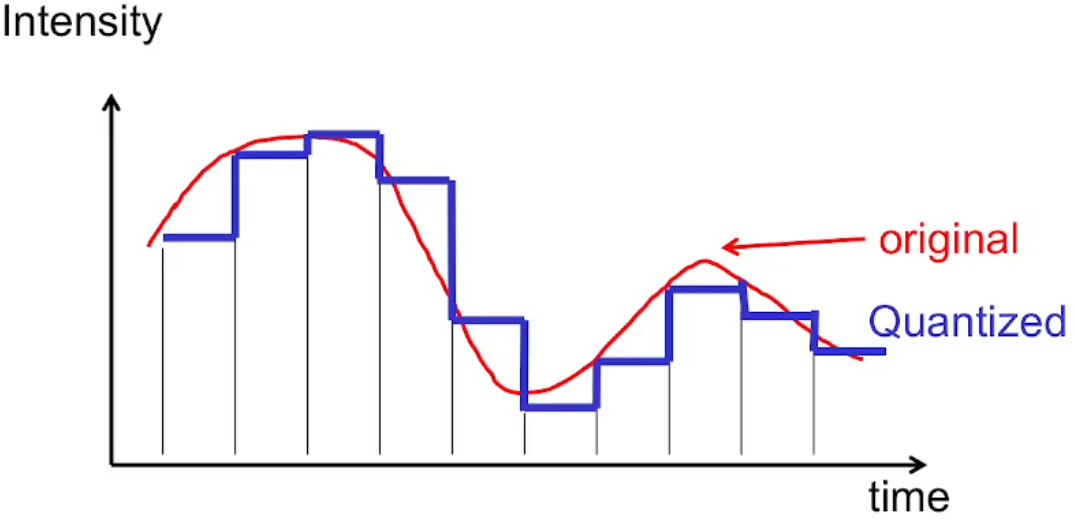
\includegraphics[width=12cm,height=3.5cm,keepaspectratio]{01_3.png}}
				\end{figure}
				\\La tecnica più semplice è la \textbf{quantizzazione uniforme} (o \textbf{lineare}): l'intervallo dei possibili valori viene diviso in intervalli della stessa dimensione.
				\newpage 
				\noindent 
				Notare che spesso viene persa informazione perché si arrotonda il valore del segnale e che, ovunque cada il valore quantizzato, l'accuratezza dell'operazione è sempre la stessa.
				\\Quando si progetta un quantizzatore bisogna fare in modo che il range operativo sia massimo (per catturare "valori estremi") e che la distanza dei livelli di quantizzazione sia minima (per ridurre l'errore di quantizzazione).
				\begin{figure}[ht!]
					\centering{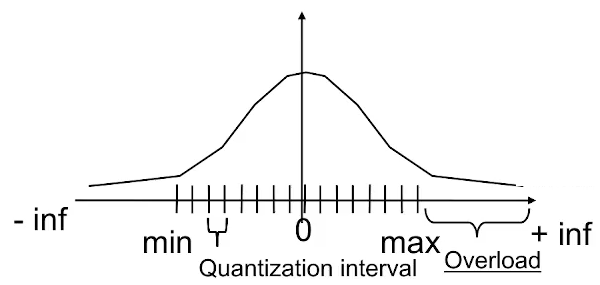
\includegraphics[width=12cm,height=3.5cm,keepaspectratio]{01_5.png}}
				\end{figure}
				\\In caso di \textbf{overload} (il valore del segnale è maggiore del massimo o minore del minimo dell'operational range) il segnale viene associato al valore max o min. Per scegliere la dimensione dell'operational range si usa la seguente regola:
				\begin{center}
					\textbf{operational range} = \textbf{4$\sigma$}
				\end{center}
				La differenza tra il valore assegnato dal quantizzatore e quello effettivo è detto \textbf{errore di quantizzazione}. Considerando questo valore come un \textbf{rumore}, è possibile includerlo nel \textbf{Rapporto Segnale/Rumore} (\textbf{SNR} = \textbf{Signal-to-Noise Ratio}, 40-50 dB è già un buon audio). In realtà il SNR è più utile se calcolato comparando la potenza del segnale più che la tensione (in dB):
				\begin{center}
					\textit{SNR = 10 $log_{10}(\sigma^{2}_{v}/\sigma^{2}_{e})$}
				\end{center}
				\begin{itemize}
					\item $\sigma^{2}_{v}$ = varianza del segnale (da gaussiana);
					\item $\sigma^{2}_{e}$ = varianza del rumore (dipende dal quantizzatore).
				\end{itemize}
				Assumendo che il rumore di quantizzazione abbia distribuzione uniforme, si ha:
				\begin{center}
					\textit{SNR $\sim$ 6*N - f($sigma^{2}_{v}/X^{2}_{max}$)}
				\end{center}
				\begin{itemize}
					\item N = numero bit;
					\item $X_{max}$ = range di quantizzazione;
					\item notare che il SNR vale 6*N solo in condizioni ottimali, ovvero solo quando viene sfruttato tutto il range del quantizzatore (quando il quantizzatore ha un range uguale alla varianza del segnale). Per esempio, se si ha un range di 10 V e il segnale in ingresso è di mV, il SNR è alto.
				\end{itemize}
				Quando si progetta un quantizzatore bisogna scegliere:
				\begin{itemize}
					\item il range operativo (valori di fondoscale);
					\item il SNR desiderato quando è usato l'intero range operativo.
				\end{itemize}

				
			\subsubsection{PCM (Pulse Code Modulation)}
				Un \textbf{Modulatore a Impulsi Codificati} (PCM) è un dispositivo in grado di campionare il segnale e di quantizzarlo su N bit per campione. Per esempio 12 bit per la telefonia e 16 bit per i CD audio. Maggiore è il numero di bit, maggiore è il SNR e, di conseguenza, il ruomore è meno fastidioso.
				\\Vediamo degli esempi sulla frequenza di trasmissione di un PCM lineare:
				\begin{itemize}
					\item CD Audio: 44100 * 16 * 2 = 1,411,200 bit/s
					\begin{itemize}
						\item 44100 = 2 * $f_{max}$;
						\item 16 = bit quantizzazione;
						\item 2 = numero di canali (cassa dx e sx);
					\end{itemize}
					\item Telefono: 8000 * 12 = 96,000 bit/s;
					\begin{itemize}
						\item 8000 = 2 * $f_{max}$ (voce udibile, inoltre la frequenza massima è stata leggermente tagliata);
					\end{itemize}
					\item Video: 720 * 576 * 8 * 30 = 100 Mbit/s;
					\begin{itemize}
						\item 720 * 576 = risoluzione (pixel);
						\item 8 = per colore;
						\item 30 = fps;
					\end{itemize}
				\end{itemize}
				
		\subsection{Codifica della Voce}
			
			\subsubsection{Voce Telefonica}
				Come visto in precedenza, la voce umana va dai 100 Hz ai 5-7 kHz circa. Per avere un'applicazione telefonica (intelligibilità = chiarezza interpretativa) decente però, non è necessario coprire interamente questo range, anche se si perde parte della naturalezza del discorso. Per questo vengono trasportate le frequenze tra i \textbf{300 Hz} e i \textbf{3400 Hz}. I valori inferiori ai 300 Hz vengono tagliati perché più che trasportare informazioni trasportano energia, con conseguenti consumi inutili. I valori oltre i 3400 Hz invece non risulatano necessari per comprendere il messaggio. Inoltre, maggiore è la distanza, minore è la frequenza trasportabile.
				\\Col passaggio dalla telefonia analogica a quella digitale, non sono cambiati questi parametri e si è decisi di usare \textbf{$F_{c}$} = \textbf{8000} Hz ($>$ 2*3400) e quantizzazione uniforme con valori a \textbf{12 bit}. Di conseguenza, la frequenza di trasmissione è di 12*8000 = 96 kbit/s.

			\newpage
			\subsubsection{Quantizzatore Uniforme}
				La tecnica più semplice é la quantizzazione uniforme (o lineare): l’intervallo dei possibili valori viene diviso in intervalli della stessa dimensione. Questa tecnica risulta ottimale (minimizza il rumore di quantizzazione) se il segnale ha densità di probabilità (pdf) uniforme all'interno del range operativo del quantizzatore (le frequenze si presentano tutte con la stessa frequenza), cosa assai rara.
				\begin{figure}[ht!]
					\centering{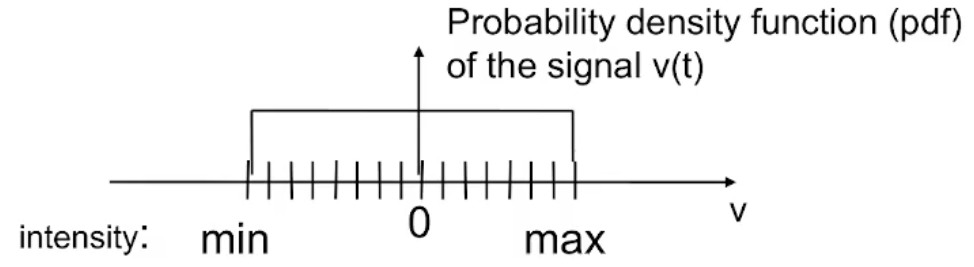
\includegraphics[width=12cm,height=2cm,keepaspectratio]{01_6.png}}
				\end{figure}

			\subsubsection{Quantizzatore Non Uniforme}
				Poichè la pdf della voce umana non è una distribuzione uniforme ma una \textbf{distribuzione gamma} (simile a gaussiana ma più "a punta"), è meglio avere più intervalli dove il segnale è più probabile. Per questo motivo è stata introdotta la quantizzazione non uniforme.
				\begin{figure}[ht!]
					\centering{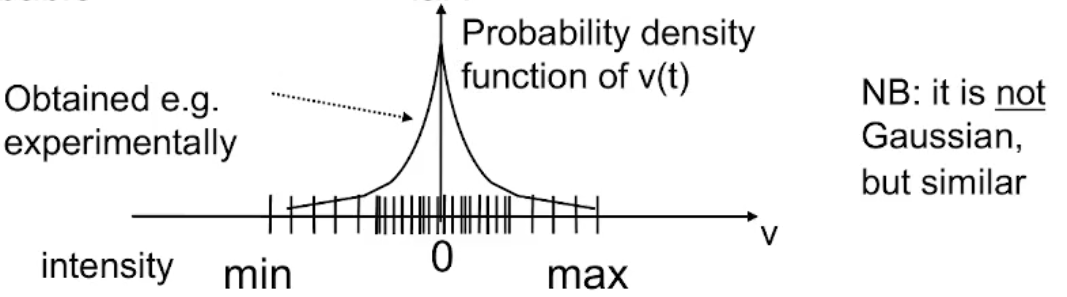
\includegraphics[width=12cm,height=2.2cm,keepaspectratio]{01_7.png}}
				\end{figure}
				\\Per calcolare l'intervallo della distribuzione che fornisce il massimo SNR viene utilizzato un algoritmo che deriva dal il \textbf{teorema di Max-Lloyd}. Applicando questo algoritmo al segnale vocale, si è riusciti ad ottenere lo stesso SNR che si otteneva con 12/16 bit usando solo 8 bit. Per questo, la \textbf{ITU} (International Telecommunication Union) ha definito uno standard (\textbf{ITU-T G711}): voce telefonica a 64 kbit/s (8 bit, $F_{c}$ = 8 kHz) e quantizzatore \textbf{log-PCM} (Pulse Code Modulation). In realtà questo standard non definisce come costruire il quantizzatore ma come passare da quello a 12 bit a quello a 8.
				\\Un codificatore/decodificatore Log-PCM prevede i livelli distribuiti su una scala semi-logaritmica: nella prima parte si ha corrispondenza lineare tra la scala a 12 bit e quella a 8, spostanosi verso gli estremi invece è logaritmica.
				\begin{figure}[ht!]
					\centering{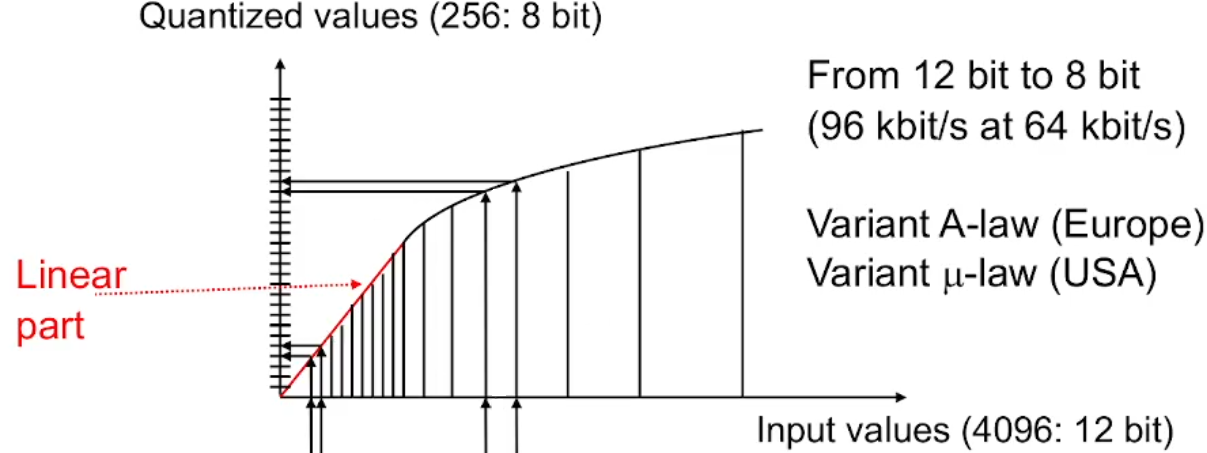
\includegraphics[width=12cm,height=2.7cm,keepaspectratio]{01_8.png}}
				\end{figure}
				\\Notare che sono presenti due varianti (una in Europa e una negli USA) e che lo standard definisce come passare da quello uniforme a 12/16 bit e non come costruire il quantizzatore perché quello uniforme è molto più facile da costruire. L'algoritmo per questa conversione risulta molto semplice e utilizza una semplice tabella di lookup per trovare il valore a 8 bit associato a quello di 12/16.
				\\Questo standard è stato utilizzato per la prima volta per le dorsali (molto più semplice gestire segnale digitale) ed è quello ancora usato per quanto rigurda la telefonia fissa (solitamente si trasmette il segnale analogico fino all'armadio di strada e poi viene codificato/decodificato).
				\\I vantaggi di questa tecnologia sono la riduzione dei bit e la semplicità (costo):
				\begin{itemize}
					\item non usa memoria: non usa RAM ma ROM;
					\item ritardo molto basso: non deve attendere N campioni ma ne codifica uno alla volta;
					\item statico: non servono algoritmi, processore\dots
				\end{itemize}

			\subsubsection{Codifica Differenziale}
				Per ridurre ulteriormente la banda rispetto al G.711 (64 kbit/s) è possibile ragionare su un gruppo di campioni anziché sul singolo campione. Per esempio, se i campioni sono molto correlati, la differenza tra due campioni consecutivi può essere rappresentata con meno bit rispetto a quelli necessari per trasmettere il valore assoluto dei campioni. La tecnica appena descritta è chiamata "codifica differenziale" e viene implementata nel \textbf{Differential PCM} (\textbf{DPCM}).
				\\Come possiamo osservare nel seguente grafico, la pdf della differenza tra due segnali ha varianza minore rispetto a quella delle frequenze assolute, di conseguenza è possibile ridurre il numero di bit. 
				\begin{figure}[ht!]
					\centering{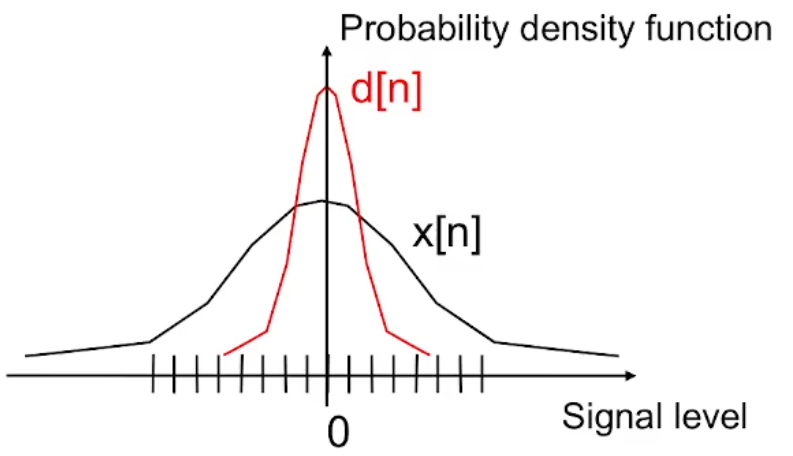
\includegraphics[width=12cm,height=3.5cm,keepaspectratio]{01_9.png}}
				\end{figure}
				\\Il lavoro eseguito da codificatore e decodificatore è il seguente:
				\begin{itemize}
					\item \textbf{encoder}: d[n] = x[n] - $\hat{x}$[n-1]
					\item \textbf{decoder}: $\hat{x}$[n] = $\hat{d}$[n] + $\hat{x}$[n-1]
				\end{itemize}
				Notare che codificatore e decodificatore usano il valore del segnale assegnato dal quantizzatore (accento circonflesso) e non quello del segnale originale.

				\paragraph{Predizione nei DPCM\\}
					\noindent Da ulteriori studi sui segnali, ci si è accorti che non tutti i valori dei campioni $\hat{x}$[n-1] hanno la stessa "importanza", per questo è stato introdotto un \textbf{coefficiente di predizione \textit{$\alpha$}}.
					\\Le performance del DPCM sono massimizzate quando la varianza dell'errore di predizione è minima:
					\begin{figure}[ht!]
						\centering{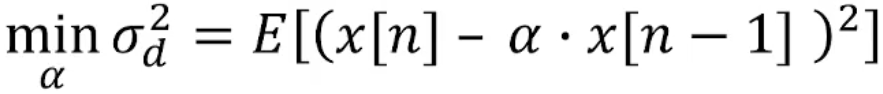
\includegraphics[width=12cm,height=0.8cm,keepaspectratio]{01_10.png}}
					\end{figure}
					\\Attraverso alcuni calcoli (non importanti a differenza della formula finale) si ottiene:
					\begin{figure}[ht!]
						\centering{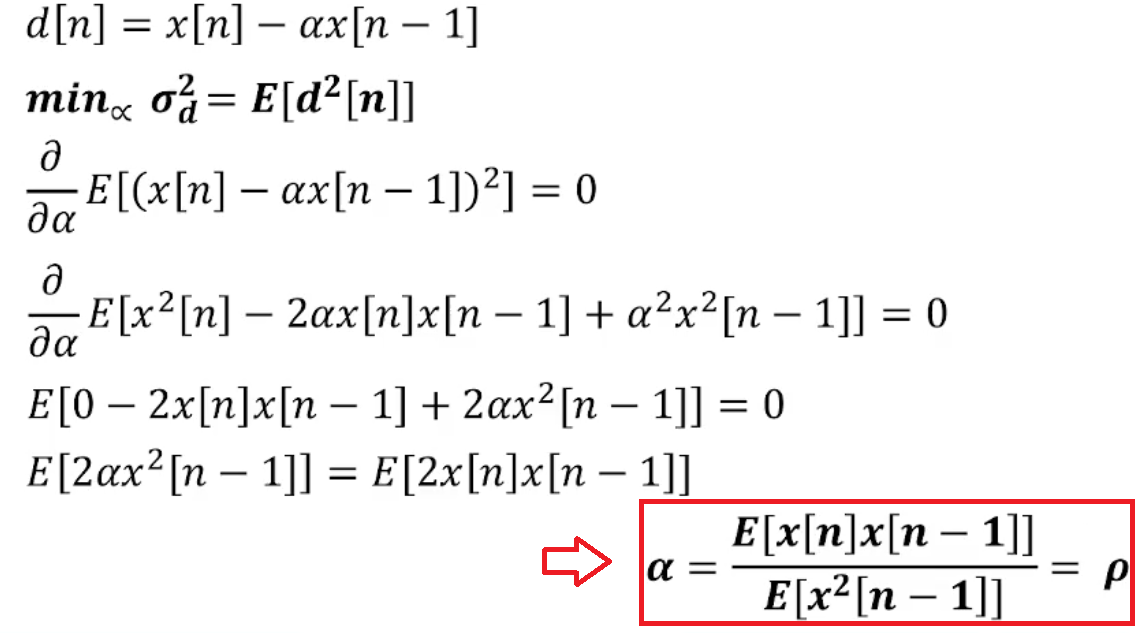
\includegraphics[width=12cm,height=4.5cm,keepaspectratio]{01_11.png}}
					\end{figure}
					\\Ovvero, \underline{per massimizzare le prestazioni, \textit{$\alpha$} deve essere uguale al coefficiente di} \\\underline{correlazione \textit{$\rho$}}.
					\\Notare che \textit{$\alpha$} è sempre compreso tra 0 e 1 e che questo è un risultato generale che vale per tutti i tipi di segnali.
					\\Il valore tipico di \textit{$\rho$} per il segnale vocale è 0.9 (il 90\% del campione corrente può essere predetto dal precedente).

				\paragraph{DPCM di Ordine N-esimo\\}
					Il ragionamento descritto nel paragrafo precedente può essere esteso considerando \textit{N} campioni precedenti all'attuale (\textbf{DPCM di ordine N-esimo}), per migliorare la predizione:
					\begin{figure}[ht!]
						\centering{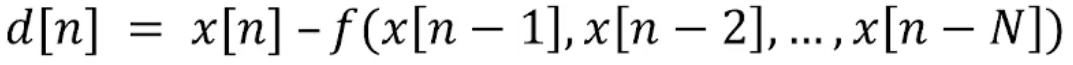
\includegraphics[width=12cm,height=0.5cm,keepaspectratio]{01_12.png}}
					\end{figure}
					\\Se f() è una combinazione lineare:
					\begin{figure}[ht!]
						\centering{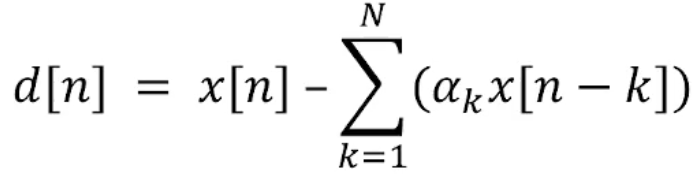
\includegraphics[width=12cm,height=1.4cm,keepaspectratio]{01_13.png}}
					\end{figure}
					\\Notare che i coefficienti sono diversi in base al campione.
					\\Per scegliere i valori dei coefficienti si usa l'\textbf{algoritmo di Levinson-Durbin}.
					\\Il valore di \textit{N} tipicamente usato per il segnale vocale in banda telefonica è tra gli 8 e i 12.

				\paragraph{Predizione Lineare}
					I risultati ottenuti fino ad ora possono essere usati per prevedere il prossimo campione senza doverlo campionare e trasmettere la differenza di un campione rispetto alla sua predizione. Questa tecnica è chiamata "Linear Prediction".
					\begin{figure}[ht!]
						\centering{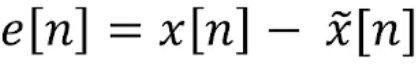
\includegraphics[width=12cm,height=0.7cm,keepaspectratio]{01_14.png}}
					\end{figure}
					\\Viene codificato solo l'errore:
					\begin{figure}[ht!]
						\centering{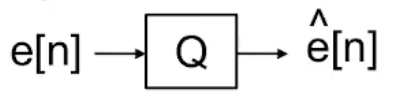
\includegraphics[width=12cm,height=1cm,keepaspectratio]{01_15.png}}
					\end{figure}
					\\La miglior predizione lineare è:
					\begin{figure}[ht!]
						\centering{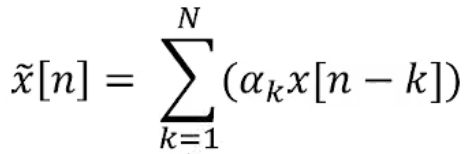
\includegraphics[width=12cm,height=1.6cm,keepaspectratio]{01_16.png}}
					\end{figure}
\end{document}